%!TEX root = ../report.tex

\section{Schnelligkeit}
Schnelligkeit ist die Fähigkeit in ermüdungsfreiem Zustand mit möglichst kurzen zeitlichem Abstand auf einen Reiz zu reagieren oder zu agieren.
\begin{figure}[H]
  \centering
  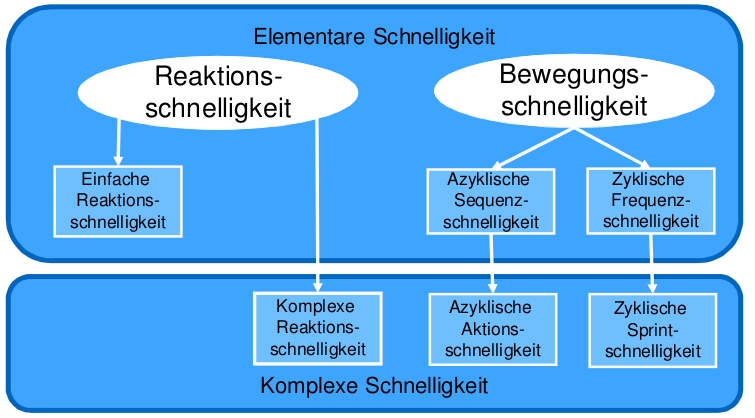
\includegraphics[width=.5\textwidth]{pictures/schnelligkeit_overview.png}
  \caption{Überblick Schnelligkeit}
\end{figure}
\begin{figure}[H]\label{fig:test}
  \centering
  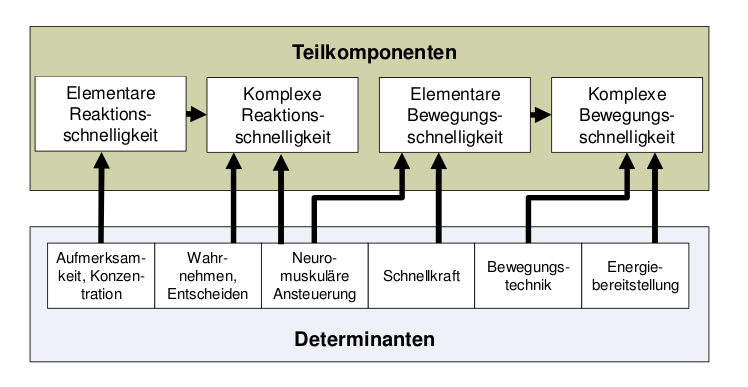
\includegraphics[width=.5\linewidth]{pictures/schnelligkeit_determinanten.png}
  \caption{Determinanten der Schnelligkei}
\end{figure}


